\documentclass[12pt,norsk,a4paper]{article}
\usepackage[norsk]{babel}
\usepackage[norsk]{isodate}
\usepackage[T1]{fontenc}
\usepackage{parskip}
\usepackage{url}
\usepackage{cancel}
\usepackage{mathtools}
\usepackage{xfrac}
\usepackage{listings}
\author{Frida Berge (fridatbe)}
\title{IN3140 --- Obligatorisk oppgave 2}
\date{\today}
\usepackage[small,euler-digits]{eulervm}
\usepackage{color}
% \usepackage{minted}
\usepackage{xcolor}
\definecolor{LightGray}{gray}{0.9}
\usepackage{a4wide}
\usepackage[top=2cm]{geometry}
\usepackage{graphicx}
\graphicspath{ {./fig/} }
\newcommand{\tuple}[1]{\ensuremath{\langle #1\rangle}}
\newcommand{\set}[1]{\ensuremath{\{#1\}}}
\newcommand{\imp}{\ensuremath{\rightarrow}}
\newcommand{\M}{\ensuremath{\mathcal{M}}}
\newcommand{\AF}{edge from parent[draw=none]}
\newcommand{\NODE}[1]{\{node \{\ensuremath{#1}\}\}}
\usepackage[explicit]{titlesec}
\titleformat{\section}{\normalfont\Large\bfseries}{}{0em}{#1\ \thesection}


\begin{document}
    \maketitle
    \renewcommand{\thesubsection}{(\alph{subsection})}
    \newpage
    \section{Task}
    \textbf{1a)} see IN3140\_task1a\_fridatbe.py\\
    \textbf{1b)} see IN3140\_task1b\_fridatbe.py\\
    \textbf{1c)} see IN3140\_task1c\_fridatbe.py\\
    \textbf{1d)} see IN3140\_task1d\_fridatbe.py\\
    \newpage

    \section{Task}
    \textbf{2a)}\\
    Because there are three links, the Jacobian will be a 6x3-matrix, and since all three joints are relovoute the Jacobian will be on the form:
    \[J = \left[ \begin{array}{ccc}
        Jv_1 & Jv_2 & Jv_3\\
        Jw_1 & Jw_2 & Jw_3\\
    \end{array} \right]
    = \left[ \begin{array}{ccc}
        z_0\times(0_3-0_0) & z_1\times(0_3-0_1) & z_2\times(0_3-0_2)\\
        z_0 & z_1 & z_2\\
    \end{array} \right]\]


    To derivate the Jacobian we have the calculations of the Denavit Hartenberg matrixes from manditory assignment 1:
   
    \[H_1^0H_2^1H_3^2 = 
            \left[ \begin{array}{cccc}
                c_1 & 0 & -s_1 & 0 \\
                s_1 & 0 & c_1 & 0 \\
                0 & -1 & 0 & d_1 \\
                0 & 0 & 0 & 1 \\
            \end{array} \right]
            \left[ \begin{array}{cccc}
                c_2 & -s_2 & 0 & a_2c_2 \\
                s_2 & c_2 & 0 & a_2s_2 \\
                0 & 0 & 1 & 0 \\
                0 & 0 & 0 & 1 \\
            \end{array} \right]
            \left[ \begin{array}{cccc}
                c_3 & -s_3 & 0 & a_3c_3 \\
                s_3 & c_3 & 0 & a_3s_3 \\
                0 & 0 & 1 & 0 \\
                0 & 0 & 0 & 1 \\
            \end{array} \right]\]
        

        \[(H_1^0H_2^1)H_3^2 = H_2^0H_3^2 =
        \left[ \begin{array}{cccc}
            c_1c_2 & -s_2c_1 & -s_1 & a_2c_1c_2 \\
            s_1c_2 & -s_1s_2 & c_1 & a_2c_2s_1 \\
            -s_2 & -c_2 & 0 & -a_2s_2+d_1 \\
            0 & 0 & 0 & 1 \\
        \end{array} \right]
        \left[ \begin{array}{cccc}
            c_3 & -s_3 & 0 & a_3c_3 \\
            s_3 & c_3 & 0 & a_3s_3 \\
            0 & 0 & 1 & 0 \\
            0 & 0 & 0 & 1 \\
        \end{array} \right]\]


            \[H_3^0 = 
            \left[ \begin{array}{cccc}
            c_1c_2c_3-c_1s_2s_3 & -c_1c_2s_3-c_1s_2c_3 & -s_1 & a_3c_1c_2c_3-a_3c_1s_2s_3+a_2c_1c_2 \\
            s_1c_2c_3-s_1s_2s_3 & -s_1c_2s_3-s_1s_2c_3 & c_1 & a_3s_1c_2c_3-a_3s_1s_2s_3+a_2s_1c_2 \\
            -s_2c_3-c_2s_3 & s_2s_3-c_2c_3 & 0 & -a_3s_2c_3-a_3c_2s_3-a_2s_2+d_1 \\
            0 & 0 & 0 & 1 \\
            \end{array} \right]\]
    From the matrixes we can read the values of ($z_0$ and $0_0$ is always the same):\\
    \[Jw_1 = z_0 = \underline{\left[\begin{array}{c}
        0 \\ 0 \\ 1
    \end{array}\right]}
    \hspace{20mm}
    Jw_2 = z_1 = \underline{\left[\begin{array}{c}
        -s_1 \\ c_1 \\ 0
    \end{array}\right]}
    \hspace{20mm}
    Jw_3 = z_2 = \underline{\left[\begin{array}{c}
        -s_1 \\ c_1 \\ 0
    \end{array}\right]}\]

    \[0_0 = \left[\begin{array}{c}
        0 \\ 0 \\ 0
    \end{array}\right]
    \hspace{5mm}
    0_1 = \left[\begin{array}{c}
        0 \\ 0 \\ d_1
    \end{array}\right]
    \hspace{5mm}
    0_2 = \left[\begin{array}{c}
        a_2c_1c_2 \\ a_2s_1c_2 \\ -a_2s_2+d_1
    \end{array}\right]\]
    \[0_3 = \left[\begin{array}{c}
        a_3c_1c_2c_3-a_3c_1s_2s_3+a_2c_1c_2 \\ a_3s_1c_2c_3-a_3s_1s_2s_3+a_2s_1c_2 \\ -a_3s_2c_3-a_3c_2s_3-a_2s_2+d_1
    \end{array}\right] = 
    \left[\begin{array}{c}
        a_3c_1c_{23}+a_2c_1c_2 \\ a_3s_1c_{23}+a_2s_1c_2 \\ -a_3s_{23}-a_2s_2+d_1
    \end{array}\right]\]

    \newpage
    Calcultaing the values of the jacobian:\\
    \[Jv_1 = z_0\times(0_3-0_0) = \left[\begin{array}{c} 0 \\ 0 \\ 1\end{array}\right]\times\left(\left[\begin{array}{c}a_3c_1c_{23}+a_2c_1c_2 \\  a_3s_1c_{23}+a_2s_1c_2 \\ -a_3s_{23}-a_2s_2+d_1\end{array}\right]-\left[\begin{array}{c}0 \\ 0 \\ 0\end{array}\right]\right) \]
    \[Jv_1 = \underline{\left[\begin{array}{c}  -a_3s_1c_{23}-a_2s_1c_2 \\ a_3c_1c_{23}+a_2c_1c_2 \\ 0\end{array}\right]}\]
    \vspace{6mm}


    \[Jv_2 = z_1\times(0_3-0_1) = \left[\begin{array}{c}-s_1 \\ c_1 \\ 0\end{array}\right]\times\left(\left[\begin{array}{c}a_3c_1c_{23}+a_2c_1c_2 \\  a_3s_1c_{23}+a_2s_1c_2 \\ -a_3s_{23}-a_2s_2+d_1\end{array}\right]-\left[\begin{array}{c}0 \\ 0 \\ d_1\end{array}\right]\right) \]
    \[= \left[\begin{array}{c}-s_1 \\ c_1 \\ 0\end{array}\right]\times\left[\begin{array}{c}a_3c_1c_{23}+a_2c_1c_2 \\  a_3s_1c_{23}+a_2s_1c_2 \\ -a_3s_{23}-a_2s_2\end{array}\right] = \left[\begin{array}{c} c_1(-a_3s_{23}-a_2s_2) \\ s_1(-a_3s_{23}-a_2s_2) \\ -s_1( a_3s_1c_{23}+a_2s_1c_2)-c_1(a_3c_1c_{23}+a_2c_1c_2)\end{array}\right]\]
    \[= \left[\begin{array}{c} -a_3c_1s_{23}-a_2c_1s_2 \\ -a_3s_1s_{23}-a_2s_1s_2\\ -a_3s_1^2c_{23}-a_2s_1^2c_2-a_3c_1^2c_{23}-a_2c_1^2c_2\end{array}\right] = \left[\begin{array}{c} -a_3c_1s_{23}-a_2c_1s_2 \\ -a_3s_1s_{23}-a_2s_1s_2\\ s_1^2(-a_3c_{23}-a_2c_2)+c_1^2(-a_3c_{23}-a_2c_2)\end{array}\right]\]
    \[Jv_2= \left[\begin{array}{c} -a_3c_1s_{23}-a_2c_1s_2 \\ -a_3s_1s_{23}-a_2s_1s_2\\ (c_1^2+s_1^2)(-a_3c_{23}-a_2c_2)\end{array}\right] = \underline{\left[\begin{array}{c} -a_3c_1s_{23}-a_2c_1s_2 \\ -a_3s_1s_{23}-a_2s_1s_2\\ -a_3c_{23}-a_2c_2\end{array}\right]}\]


    \vspace{6mm}
    \[Jv_3 = z_2\times(0_3-0_2) = \left[\begin{array}{c}-s_1 \\ c_1 \\ 0\end{array}\right]\times\left(\left[\begin{array}{c}a_3c_1c_{23}+a_2c_1c_2 \\  a_3s_1c_{23}+a_2s_1c_2 \\ -a_3s_{23}-a_2s_2+d_1\end{array}\right]-\left[\begin{array}{c}a_2c_1c_2 \\ a_2s_1c_2 \\ -a_2s_2+d_1\end{array}\right]\right) \]
    \[= \left[\begin{array}{c}-s_1 \\ c_1 \\ 0\end{array}\right]\times\left[\begin{array}{c}a_3c_1c_{23} \\  a_3s_1c_{23} \\ -a_3s_{23}\end{array}\right] = \left[\begin{array}{c} c_1(-a_3s_{23}) \\ s_1(-a_3s_{23}) \\ -s_1( a_3s_1c_{23})-c_1(a_3c_1c_{23})\end{array}\right] = \left[\begin{array}{c} -a_3c_1s_{23} \\ -a_3s_1s_{23}\\ -a_3s_1^2c_{23}-a_3c_1^2c_{23}\end{array}\right]\]
    \[Jv_3=  \left[\begin{array}{c} -a_3c_1s_{23} \\ -a_3s_1s_{23}\\ s_1^2(-a_3c_{23})+c_1^2(-a_3c_{23})\end{array}\right]=\underline{\left[\begin{array}{c} -a_3c_1s_{23} \\ -a_3s_1s_{23}\\ -a_3c_{23}\end{array}\right]}\]

    \vspace{6mm}
    \[J = \underline{\left[\begin{array}{ccc}
        -a_3s_1c_{23}-a_2s_1c_2 & -a_3c_1s_{23}-a_2c_1s_2 & -a_3c_1s_{23}\\
        a_3c_1c_{23}+a_2c_1c_2 & -a_3s_1s_{23}-a_2s_1s_2 & -a_3s_1s_{23}\\
        0 & -a_3c_{23}-a_2c_2 & -a_3c_{23}\\
        0 & -s_1 & -s_1\\
        0 & c_1 & c_1\\
        1 & 0 & 0
    \end{array}\right]} \]


    \newpage
    \textbf{2b)}\\
    % What do we call configurations for which rank J(q) is less than the maximum value?
    When the rank of J(q) (number of lineary independent columns in J) is lower than the maximum value (number of columns in J) we have a singular configuration.
    Because then we have lineary dependent columns in the matrix and there would be either zero or infinitly many solutions to the inverse kinematics.\\

    \textbf{2c)}\\
    % Use the Jacobian matrix to find the singular configurations for the robot.
    % Finner når det(Jv) = 0 for da er matisen singulær
    % Method 1:\\
    % The maximum is the number of columns in Jv, which is 3, and the rank of Jv(q) is the number of lineary independent columns in Jv.
    % hvis alle kolonnene er lineært uavhengige er det ikke en sigulær konfig (det er en singulært konfig hvis det fins uendelig eller ingen løsninger på inverskinematikken)\\
    % Method 2:\\
    % When the determinant of this matrix equals zero the configuration is singular:\\
    % Method 3:\\
    % view the robot
    By solving the expressions be setting the determinant of the Jacobian to zero we will find the singular configurations (we only view the Jv-matix, where we get the velocity in each of the coordinate's directions):
    \[det(Jv) =det\left( \left[\begin{array}{ccc}
        -a_3s_1c_{23}-a_2s_1c_2 & -a_3c_1s_{23}-a_2c_1s_2 & -a_3c_1s_{23}\\
        a_3c_1c_{23}+a_2c_1c_2 & -a_3s_1s_{23}-a_2s_1s_2 & -a_3s_1s_{23}\\
        0 & -a_3c_{23}-a_2c_2 & -a_3c_{23}\\
    \end{array}\right]\right) = 0\]

    Part A:
    \[-a_3s_1c_{23}-a_2s_1c_2\left|\begin{array}{cc}
        -a_3s_1s_{23}-a_2s_1s_2 & -a_3s_1s_{23}\\
        -a_3c_{23}-a_2c_2 & -a_3c_{23}\\
    \end{array}\right|\]

    Part B:
    \[a_3c_1c_{23}+a_2c_1c_2 \left|\begin{array}{cc}
        -a_3c_1s_{23}-a_2c_1s_2 & -a_3c_1s_{23}\\
        -a_3c_{23}-a_2c_2 & -a_3c_{23}\\
    \end{array}\right|\]
    Part C:
    \[0\left|\begin{array}{cc}
        -a_3c_1s_{23}-a_2c_1s_2 & -a_3c_1s_{23}\\
        -a_3s_1s_{23}-a_2s_1s_2 & -a_3s_1s_{23}\\
    \end{array}\right| = 0\]
    Since part C equals 0, all we have to find is the values for when part A equals part B, because then det(Jv) = A-B = 0:\\
    Starting with part A:
    \[-a_3s_1c_{23}-a_2s_1c_2[(-a_3s_1s_{23}-a_2s_1s_2)(-a_3c_{23})-(-a_3s_1s_{23})(-a_3c_{23}-a_2c_2)]\]
    \[-a_3s_1c_{23}-a_2s_1c_2[(a_3^2c_{23}s_1s_{23}+a_2a_3c_{23}s_1s_2)-(a_3^2c_{23}s_1s_{23} + a_2a_3c_2s_1s_{23})]\]
    \[-a_3s_1c_{23}-a_2s_1c_2[(\cancel{a_3^2c_{23}s_1s_{23}}+a_2a_3c_{23}s_1s_2)-(\cancel{a_3^2c_{23}s_1s_{23}} + a_2a_3c_2s_1s_{23})]\]
    \[-a_3s_1c_{23}-a_2s_1c_2[a_2a_3c_{23}s_1s_2-a_2a_3c_2s_1s_{23}]\]
    \[-a_2a_3^2c_{23}^2s_1^2s_2 + a_2a_3^2c_2c_{23}s_1^2s_{23} - a_2^2a_3c_2c_{23}s_1^2s_2 +a_2^2a_3c_2^2s_1^2s_{23}\]
    \[-a_2a_3^2c_{23}^2s_1^2s_2 + a_2a_3^2c_2c_{23}s_1^2s_{23} - a_2^2a_3c_2c_{23}s_1^2s_2 +a_2^2a_3c_2^2s_1^2s_{23}\]


    Then part B:
    \[a_3c_1c_{23}+a_2c_1c_2[(-a_3c_1s_{23}-a_2c_1s_2)(-a_3c_{23})-(-a_3c_1s_{23})(-a_3c_{23}-a_2c_2)]\]
    \[a_3c_1c_{23}+a_2c_1c_2[\cancel{a_3^2c_1c_{23}s_{23}}+a_2a_3c_1c_{23}s_2 - (\cancel{a_3^2c_1c_{23}s_{23}}+a_2a_3c_1c_2s_{23})]\]
    \[a_3c_1c_{23}+a_2c_1c_2[a_2a_3c_1c_{23}s_2 -a_2a_3c_1c_2s_{23}]\]
    \[a_2a_3^2c_1^2c_{23}^2s_2 - a_2a_3^2c_1^2c_2c_{23}s_{23} + a_2^2a_3c_1^2c_2c_{23}s_2 -a_2^2a_3c_1^2c_2^2s_{23}\]
    \[a_2a_3^2c_1^2c_{23}^2s_2 - a_2a_3^2c_1^2c_2c_{23}s_{23} + a_2^2a_3c_1^2c_2c_{23}s_2 -a_2^2a_3c_1^2c_2^2s_{23}\]
    
    Part A = Part B:\\
    \[-a_2a_3^2c_{23}^2s_1^2s_2 + a_2a_3^2c_2c_{23}s_1^2s_{23} - a_2^2a_3c_2c_{23}s_1^2s_2 +a_2^2a_3c_2^2s_1^2s_{23}\]
    \[= a_2a_3^2c_1^2c_{23}^2s_2 - a_2a_3^2c_1^2c_2c_{23}s_{23} + a_2^2a_3c_1^2c_2c_{23}s_2 -a_2^2a_3c_1^2c_2^2s_{23}\]
    \[ a_2a_3^2c_{23}^2s_2(\cancel{c_1^2+s_1^2}) - a_2a_3^2c_2c_{23}s_{23}(\cancel{c_1^2+s_1^2})+a_2^2a_3c_2c_{23}s_2(\cancel{c_1^2+s_1^2})-a_2^2a_3c_2^2s_{23}(\cancel{c_1^2+s_1^2}) = 0\]
    \[ a_2a_3^2c_{23}^2s_2 - a_2a_3^2c_2c_{23}s_{23}+a_2^2a_3c_2c_{23}s_2-a_2^2a_3c_2^2s_{23} = 0\]
    \[ a_2a_3^2c_{23}(s_2c_{23}-s_{23}c_2) + a_2^2a_3c_2(c_{23}s_2 - s_{23}c_2) = 0\]
    \[ a_2a_3^2c_{23}(s_2(c_2c_3-s_2s_3)-c_2(s_2c_3+c_2s_3)) + a_2^2a_3c_2(s_2(c_2c_3-s_2s_3) - c_2(s_2c_3+c_2s_3)) = 0\]
    \[ a_2a_3^2c_{23}(\cancel{c_2c_3s_2}-s_2^2s_3-\cancel{c_2c_3s_2}-c_2^2s_3) + a_2^2a_3c_2(\cancel{c_2c_3s_2}-s_2^2s_3 - \cancel{c_2c_3s_2}-c_2^2s_3) = 0\]
    \[ a_2a_3^2c_{23}(-s_2^2s_3-c_2^2s_3) + a_2^2a_3c_2(-s_2^2s_3-c_2^2s_3) = 0\]
    \[ a_2a_3^2c_{23}(-s_3(\cancel{s_2^2+c_2^2})) + a_2^2a_3c_2(-s_3(\cancel{s_2^2-c_2^2})) = 0\]
    \[ -s_3(a_2a_3^2c_{23} + a_2^2a_3c_2) = 0\]
    \[ -s_3 = 0 \hspace{10mm} \vee \hspace{10mm} a_2a_3(a_3c_{23} + a_2c_2) = 0 \]
    We know that $a_2$ and $a_3$ are 222.1 and 136.2, thus not zero:\\
    \[a_2a_3(a_3c_{23} + a_2c_2) = 0\]
    \[a_3c_{23} + a_2c_2 = 0\]
    \[\underline{a_3(c_2c_3-s_2s_3) + a_2c_2 = 0}\]
    And we know the value of $\theta_3$ when $sin(\theta) = 0$:\\
    \[s_3 = 0 \hspace{5mm} ->  \hspace{5mm} \theta_3 = \underline{0}  \hspace{5mm} \vee \hspace{5mm} \theta_3 = \underline{\pi}\]
    

    \textbf{2d)}\\
    % Give an evaluation of these results, and draw at least one of these singular configurations. The drawing(s) shall have a simple 3D layout like the ones in the lecture slides, see referred standard below.
    I chose to show the singularity when $\theta_3 = 0$, which makes link 2 and 3 collinear, and it would be like link 2 and 3 is one combined link.
    This makes the robot have one less degree of freedom, and therefore is defined as a singularity.
    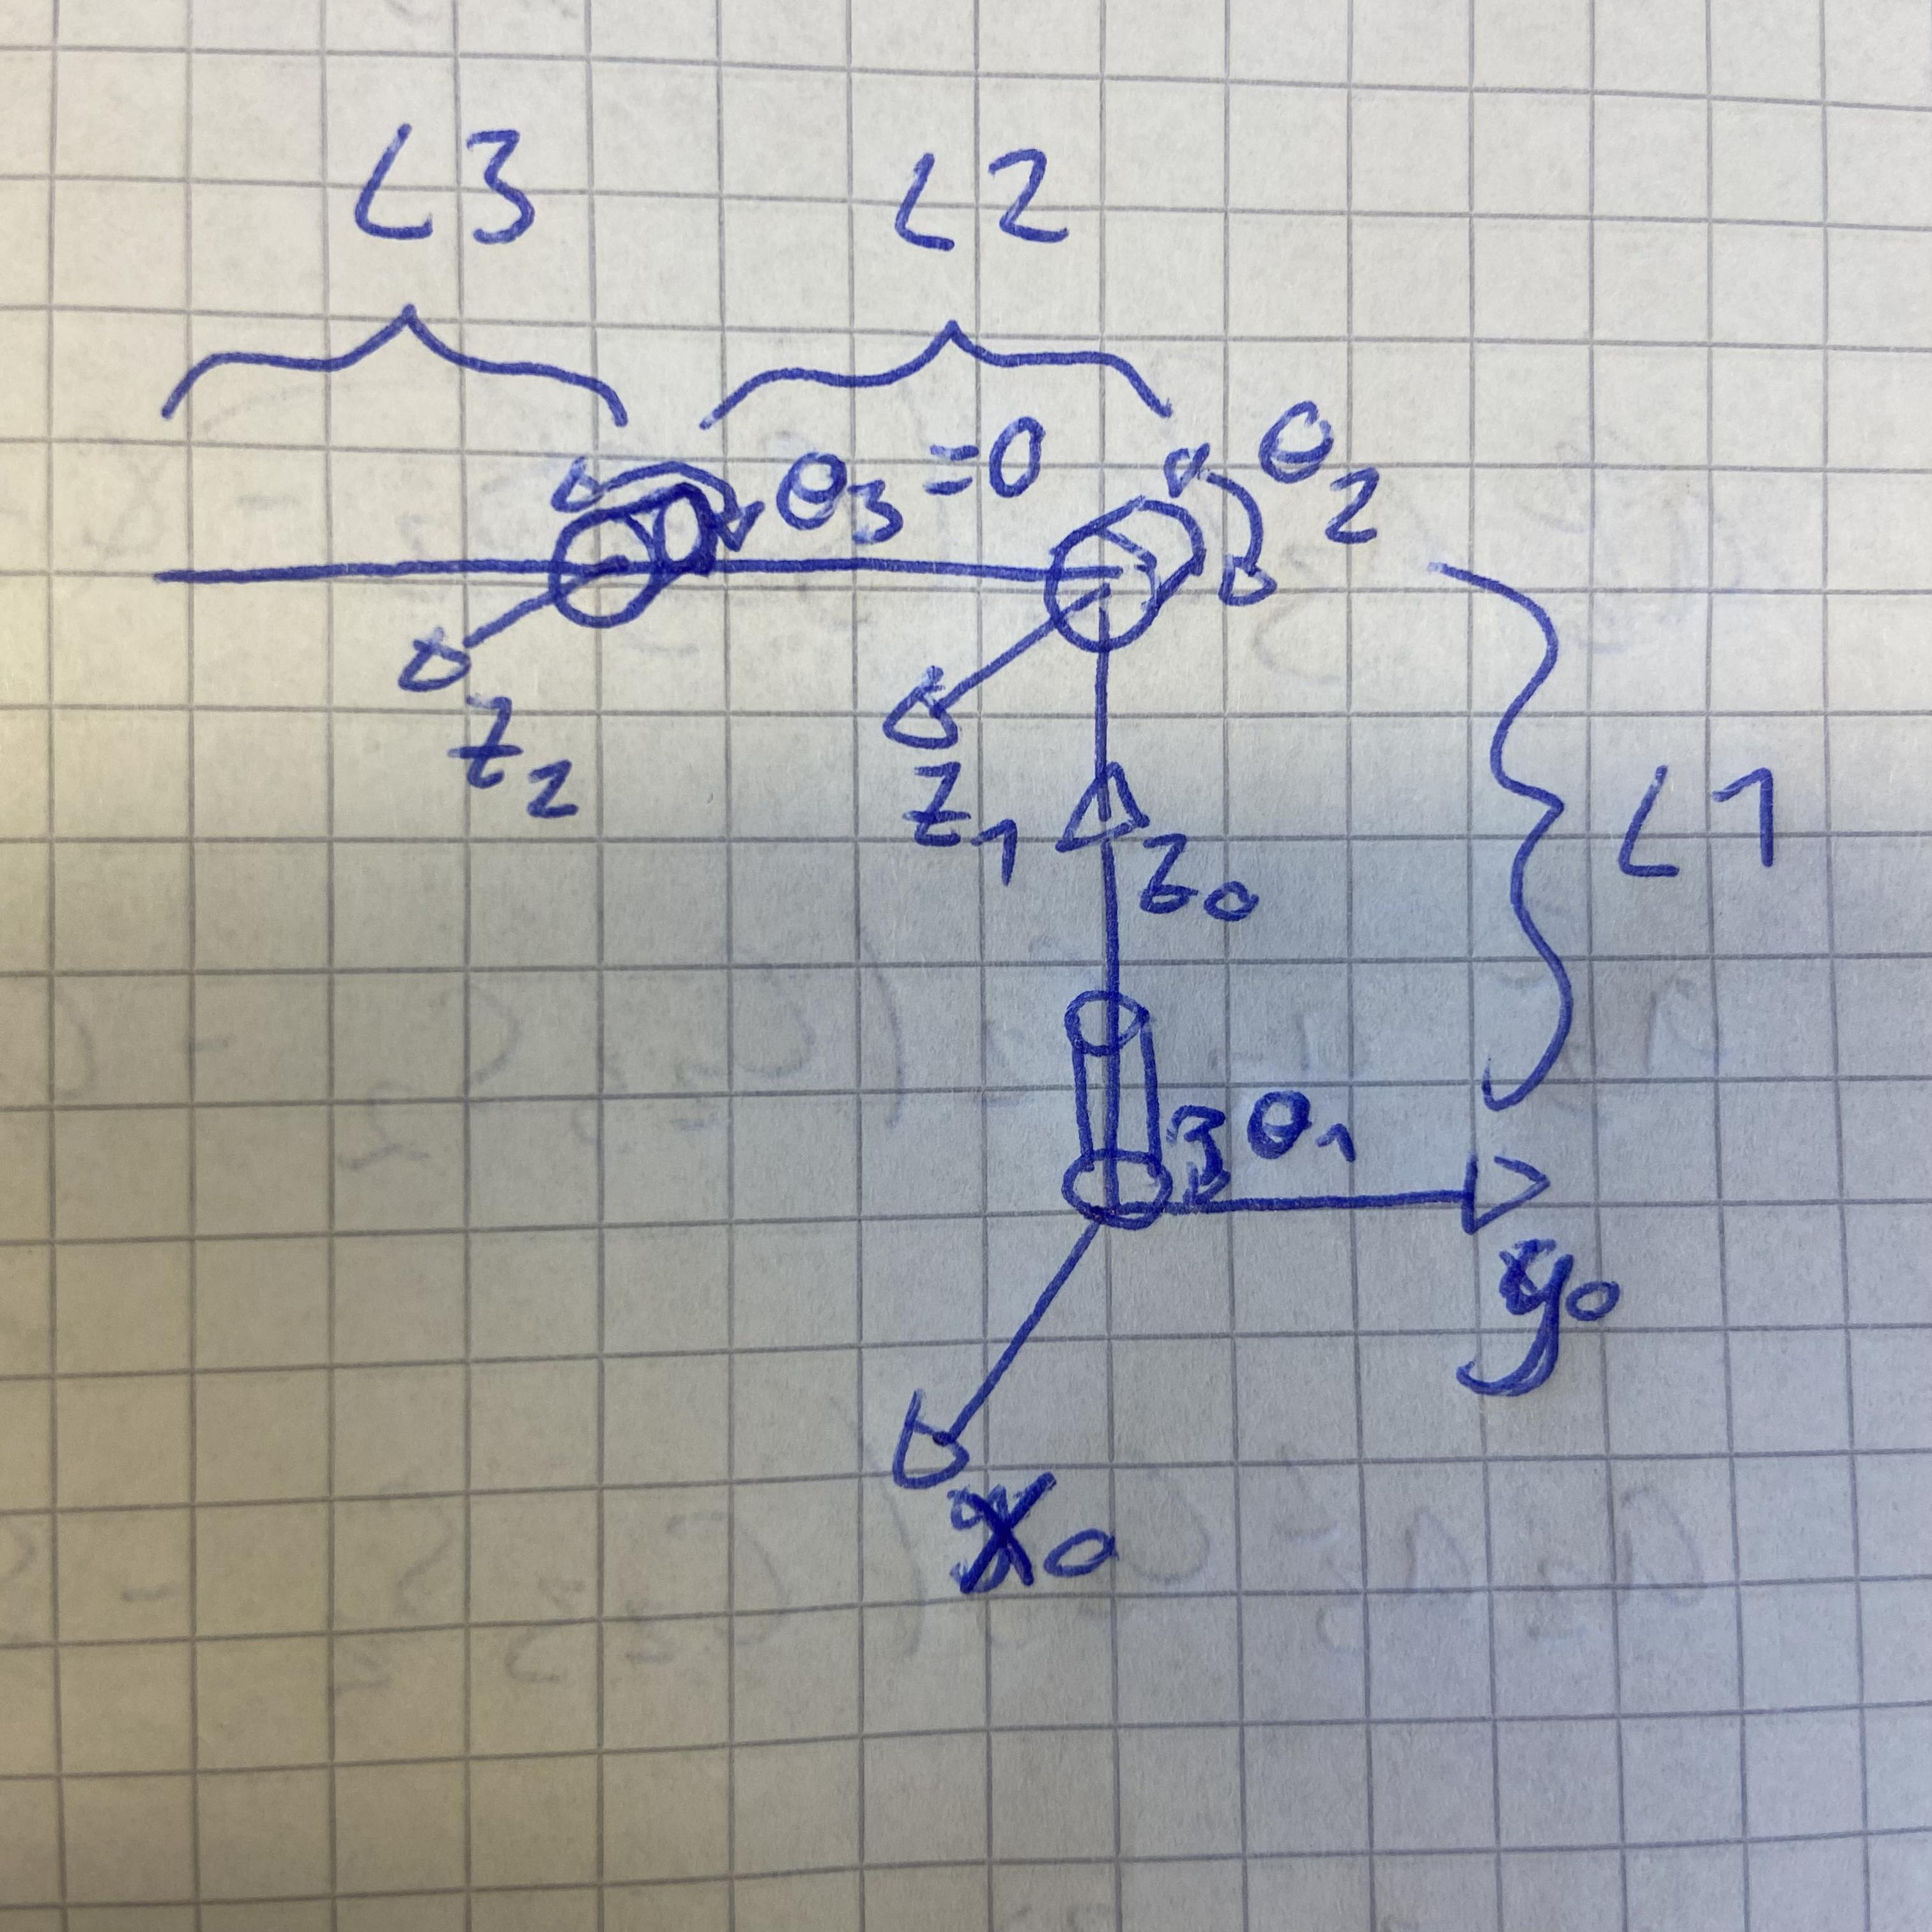
\includegraphics[width=0.5\textwidth]{sin.jpg}\\
    Viewing the two other results:
    \begin{itemize}
        \item $\theta_3 = \pi$, because the tip and link 3 will lay directly on top of link 2 (one less degree of freedom)
        \item $a_3(c_2c_3-s_2s_3) + a_2c_2 = 0$, because in this case the tip will intersect the $z_0$-axis, and there would be infinitly many solutions to the inverse kinematics because $\theta_1$ does not matter
    \end{itemize} 
    
    \textbf{2e)}\\
    % A natural extension of the simplified robot would be a spherical wrist on the end. How can a spherical wrist alone (only picturing the wrist)
    % be in singularity? Draw and explain. The drawing shall be a simple 3D illustration.
    % se fig 3.7 side 85 for tegning
    \begin{minipage}[t]{.5\textwidth}
        Example of a singularity \\
        for the spherical wrist:\\
        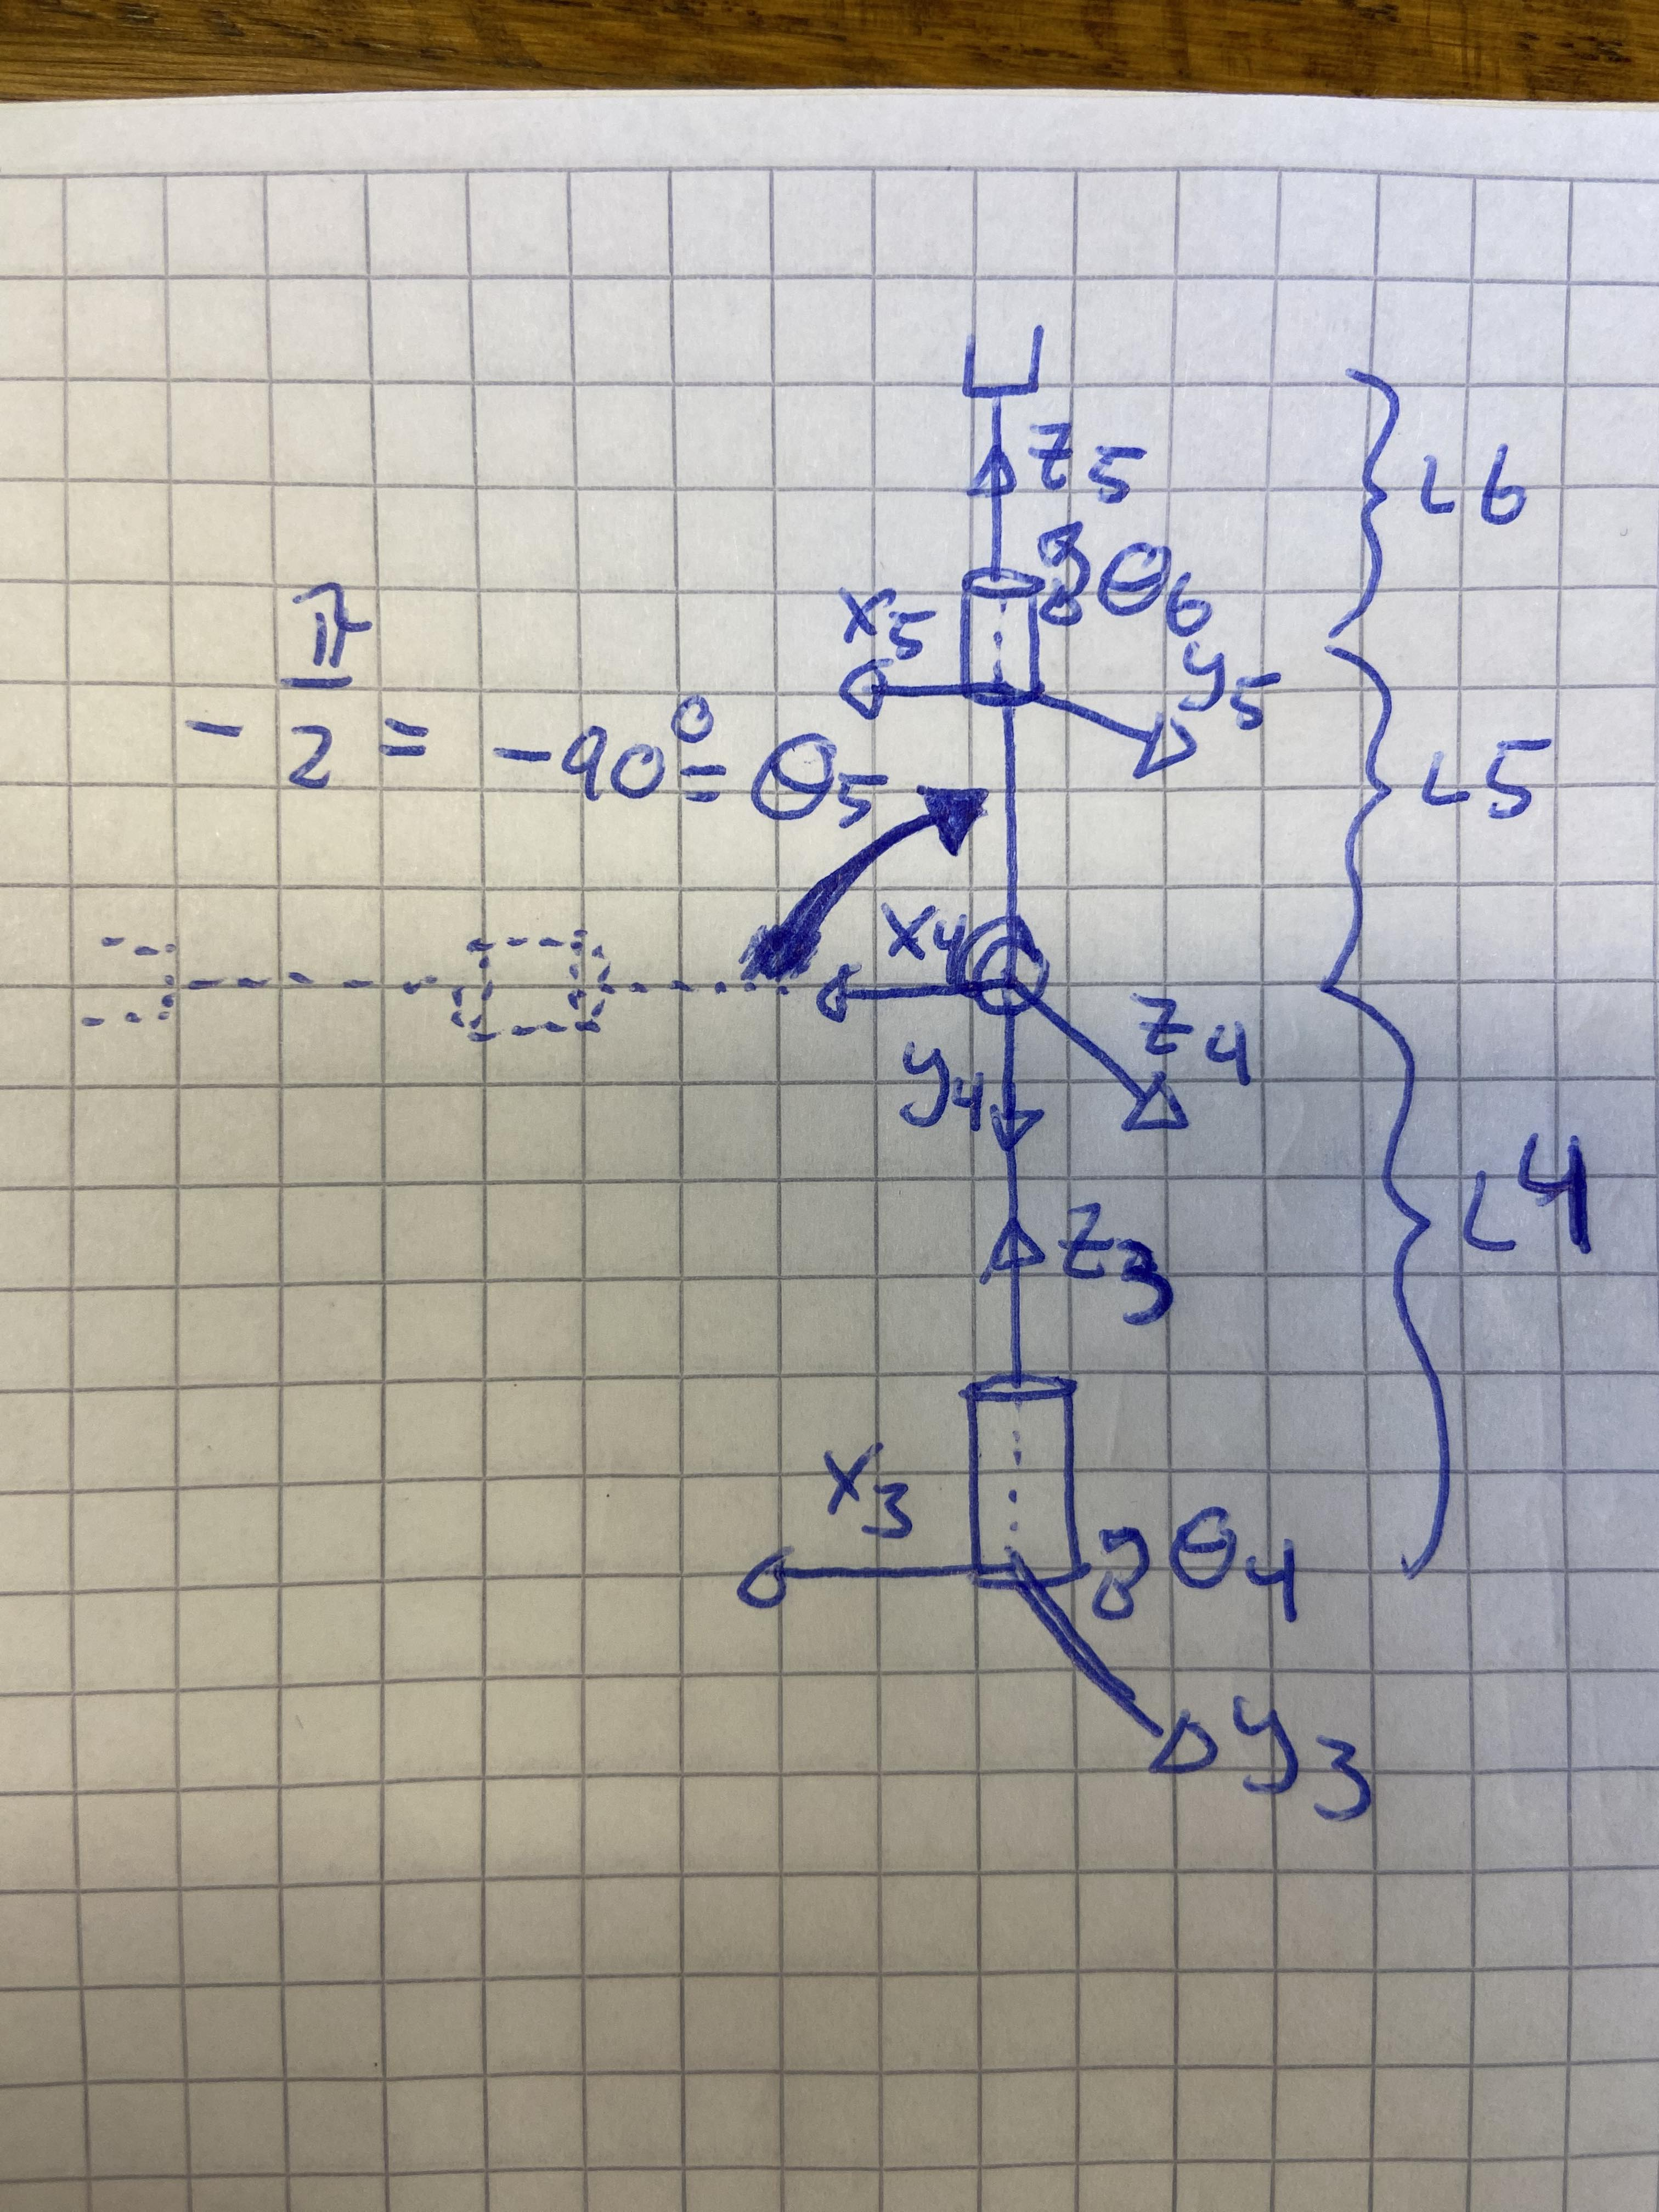
\includegraphics[width=\textwidth]{wri.jpg}
    \end{minipage}
    \hspace{5mm}
    \begin{minipage}[t]{.5\textwidth}
        % \vspace{6mm}
        This is a singularity because the $z_5$-axis and $z_3$-axis are collinear. 
        If $\theta_5 = \frac{\pi}{2}$ another singularity would appear.
        In these cases, there would be infinitly many soloutions to the inverse kinematics
        because the angle of $\theta_4$ and $\theta_6$ would not matter for the point of the gripper.\\\\
        When $\theta_5 = -90^\circ$ the wrist is limited to one less degree of freedom because it would be like link 4 and link 5 is one combined link.
        Also joint 4 and 6 would have the same effekt on the wrist (unless one or both of them were limited to less than 360 degrees of rotation),
        so this would make the gripper to have the same degree of freedom as a one-revoloute-joint wrist (DOF = 1) instead of three.
        And the same situations will appear when $\theta_5=90$, because link 6 would be placed on top of link 4 (be collinear)


    \end{minipage}\\

    \textbf{2f)}\\
    % What is the practical consequenses of not handeling singularities?
    When the robot ends up in a singular configuration, it cannot move in some direction/directions.
    This means that if the robot ends up in a singular configuration, it (the robot) might get destroyd if it tries to move in the 'impossible' direction because it would theoretically require initinite force to get out of the position.


    \newpage
    \section{Task}
    \textbf{3a)} see IN3140\_task3a\_fridatbe.py\\
    \textbf{3b)} see IN3140\_task3b\_fridatbe.py\\

        
\end{document}